% generated by research/frisos-sturm/figura_godsil.py (Curiosity); do not edit by hand
\begin{figure}[H]
\centering
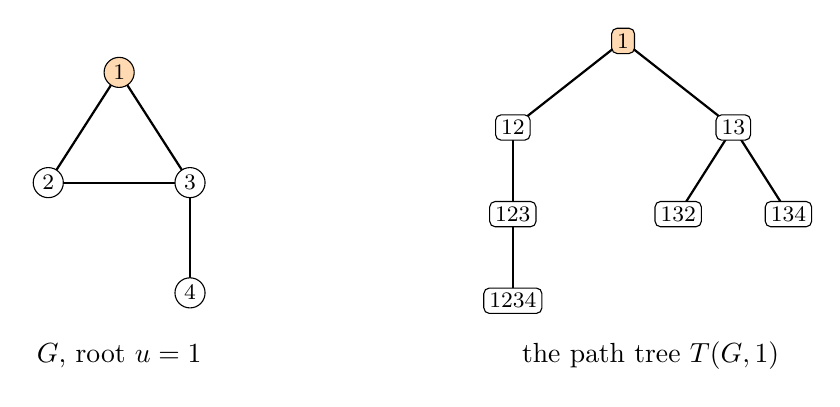
\begin{tikzpicture}[v/.style={circle, draw, fill=white, inner sep=1.5pt, font=\footnotesize}, t/.style={rounded corners=2pt, draw, fill=white, inner sep=2pt, font=\footnotesize}]
\begin{scope}[shift={(-4.2,-0.4)}]
  \draw[thick] (0.00,0.00) -- (-0.90,-1.40);
  \draw[thick] (0.00,0.00) -- (0.90,-1.40);
  \draw[thick] (-0.90,-1.40) -- (0.90,-1.40);
  \draw[thick] (0.90,-1.40) -- (0.90,-2.80);
  \node[v, fill=orange!30] at (0.00,0.00) {1};
  \node[v] at (-0.90,-1.40) {2};
  \node[v] at (0.90,-1.40) {3};
  \node[v] at (0.90,-2.80) {4};
  \node at (0,-3.6) {$G$, root $u = 1$};
\end{scope}
\begin{scope}[shift={(2.2,0)}]
  \draw[thick] (0.00,0.00) -- (-1.40,-1.10);
  \draw[thick] (0.00,0.00) -- (1.40,-1.10);
  \draw[thick] (1.40,-1.10) -- (0.70,-2.20);
  \draw[thick] (1.40,-1.10) -- (2.10,-2.20);
  \draw[thick] (-1.40,-1.10) -- (-1.40,-2.20);
  \draw[thick] (-1.40,-2.20) -- (-1.40,-3.30);
  \node[t, fill=orange!30] at (0.00,0.00) {1};
  \node[t] at (1.40,-1.10) {13};
  \node[t] at (2.10,-2.20) {134};
  \node[t] at (0.70,-2.20) {132};
  \node[t] at (-1.40,-1.10) {12};
  \node[t] at (-1.40,-2.20) {123};
  \node[t] at (-1.40,-3.30) {1234};
  \node at (0.35,-4.0) {the path tree $T(G, 1)$};
\end{scope}
\end{tikzpicture}
\caption{A graph and its path tree at vertex~1: one tree vertex for each path that starts at~1. Here $\mu(G) = x^{4} - 4 x^{2} + 1$ and $\mu(T) = x^{7} - 6 x^{5} + 9 x^{3} - 2 x = \mu(G)\,(x^{3} - 2 x)$.}
\label{fig:pathtree}
\end{figure}
